\documentclass[11pt]{amsart}

\usepackage[utf8]{inputenc}
\usepackage{amsmath}
\usepackage{physics}
\usepackage{graphicx}
\usepackage{cancel}

\renewcommand{\thesubsection}{\thesection.\alph{subsection}}

\title[Electrodynamics]{Electrodynamics \\
	\hrulefill \small{ FYS3120: Problem Set 11 } \hrulefill}

\author[Winther-Larsen]{Sebastian G. Winther-Larsen}

\date{\today}

\begin{document}

\maketitle

\section{Simple Lagrangian Dynamics}

A non-relativistic particle, with electric charge $q$ and mass $m$ moves in a magnetic dipole field, given by the vector potential
\begin{equation}
\va{A} = \frac{\mu_0}{4\pi r^3}(\va{\mu} \cp \va{r}),
\end{equation}
where $\va{\mu}$ is the magnetic dipole moment of a static charge distribution centered at the origin.

\subsection{Lagrangian}
The Lagrangian is given by
\begin{equation}
\label{eq:lagrangian1}
L = T + q\va{v} \vdot \va{A}.
\end{equation}
The kinetic energy is simply $T = \frac{1}{2}m\va{v}^2$ while the potential is
\begin{align*}
q\va{v} \vdot \va{A} &= \frac{q\mu_0}{4\pi r^3}\va{v}\vdot(\va{\mu} \cp \va{r}) \\
					 &= \frac{q\mu_0}{4\pi r^3}\va{\mu}\vdot(\va{r}\cp\va{v}) \\
					 &= \frac{q\mu_0}{4\pi m r^3}\va{\mu}\vdot\va{\ell},
\end{align*}
using the cyclic invariance of the vector triple product and $\va{\ell} = m\va{r}\cp\va{v}$. Inserting the parts into \ref{eq:lagrangian1} the Lagrangican becomes
\begin{equation}
\label{eq:lagranrian2}
L = \frac{1}{2}m\va{v}^2 + \frac{q\mu_0}{4\pi m r^3}\va{\mu}\vdot\va{\ell}.
\end{equation}

\subsection{Alternative Lagrangian}
We now make the assumption that the magnetic dipole moment is oriented along the $z$-axis and that the particle moves in the $(x,y)$-plane. In the following, $r = \abs{\va{r}}$ and  the angle $\phi$ between the $x$-axis and the position vector $va{r}$ are chosen as generalised coordinates.

With the magnetic dipole moment oriented along the z-axis, 
\begin{align*}
\va{\mu}\vdot\va{\ell} = \abs{\va{\mu}}\ell_z = \abs{\va{\mu}}(\va{r}\cp\va{p})_z = \abs{\va{\mu}}m(x\dot{y}-y\dot{x}),
\end{align*} 
where $x = r\cos\phi$ and $y = r\sin\phi$. This gives
\begin{align*}
x\dot{y} - y\dot{x} &= r\cos\phi(\dot{r}\sin\phi + r\dot{\phi}\cos\phi) \\
					&- r\sin\phi(\dot{r}\cos\phi - r\dot{\phi}\sin\phi) \\
					&= r^2\phi\cos^2\phi + r^2\phi\sin^2\phi = r^2\phi,
\end{align*} 
similarly
\begin{align*}
\dot{x} &= \dot{r}\cos\phi - r\dot{\phi}\sin\phi \\
\dot{y} &= \dot{r}\sin\phi + r\dot{\phi}\cos\phi \\
\dot{x}^2 &= \dot{r}^2\cos^2\phi - 2r\dot{r}\dot{\phi}\cos\phi\sin\phi + r^2\dot{\phi}^2\sin^2\phi \\
\dot{y}^2 &= \dot{r}^2\sin^2\phi + 2r\dot{r}\dot{\phi}\cos\phi\sin\phi + r^2\dot{\phi}^2\cos^2\phi \\
\dot{v}^2 &= \dot{x}^2 + \dot{y}^2 = \dot{r}^2 + r^2\dot{\phi}^2.
\end{align*}
The Lagrangian with generalised coordinates becomes
\begin{equation}
\label{eq:lagrangian3}
L = \frac{1}{2}m(\dot{r}^2 + \dot{r}^2\dot{\phi}^2) + \frac{q\mu_0}{4\pi mr^3}\abs{\va{\mu}}mr^2\dot{\phi} = \frac{1}{2}m(\dot{r}^2 + \dot{r}^2\dot{\phi}^2) + \lambda\frac{\dot{\phi}}{r},
\end{equation}
where $\lambda \equiv q\mu_0\abs{\va{\mu}}/4\pi$. 

The canonical momentum $p_\phi$ conjugate to $\phi$ becomes
\begin{equation}
\label{eq:conjmomphi}
p_\phi = \frac{\partial L}{\partial \dot{\phi}} = mr^2\dot{\phi} + \frac{\lambda}{r}
\end{equation}
$\phi$ is a cyclic coordinate, because the Lagrangian in equation \ref{eq:lagrangian3} does not explicityly depend on $\phi$. This implies that the conjugate momentum $p_\phi$ is constant. 

The Lagrangian in equation \ref{eq:lagrangian3} does not depend exlicitly on time $t$. This means that the Hamiltonian must be conserved
\begin{equation}
H = \dot{r}p_r + \dot{\phi}p_\phi - L = m\dot{r}^2 + mr^2\dot{\phi}^2 + \lambda\frac{\dot{\phi}}{r} - L = \frac{1}{2}m(\dot{r}^2 + r^2\dot{\phi}^2) = T.
\end{equation}
Since the Hamiltonian equals the kinetic energy and the Hamiltonian is conserved, the kinetic energy is conserved by the magnetic field.

\subsection{Kinetic Energy Conservation}
Lagrange's equation for $r$ is
\begin{equation}
\frac{d}{dt}\left(\frac{\partial L}{\partial \dot{r}}\right) - \frac{\partial L}{\partial r} = \dot{p}_r - \frac{\partial L}{\partial r} = m\ddot{r} - mr\dot{\phi}^2 + \lambda\frac{\dot{\phi}}{r^2} = 0.
\end{equation}
Here one can eliminate $\dot{\phi}$ by inserting $\dot{\phi} = \frac{p_\phi}{mr^2} - \frac{\lambda}{mr^3}$ found from equation \ref{eq:conjmomphi}. This yields
\begin{align*}
& m\ddot{r} - mr\left(\frac{p_\phi}{mr^2} + \frac{\lambda}{mr^3} \right) - \frac{\lambda}{r^2}\left(\frac{p_\phi}{mr^2} - \frac{\lambda}{mr^3}\right) \\
=& m\ddot{r} - mr\left(\frac{p_\phi^2}{m^2r^4} - \frac{2p_\phi\lambda}{m^2r^5} + \frac{\lambda^2}{m^2r^6}\right) + \frac{p_\phi\lambda}{mr^4} - \frac{\lambda^2}{mr^5} \\
=& m\ddot{r} - \frac{p_\phi^2}{mr^3} + \frac{2p_\phi\lambda}{mr^4} - \frac{\lambda^2}{mr^5} + \frac{p_\phi\lambda}{mr^4} - \frac{\lambda^2}{mr^5} = 0
\end{align*}
\begin{equation}
\label{eq:beforersquared}
\rightarrow m\ddot{r} - \frac{p_\phi^2}{mr^3} + \frac{3p_\phi\lambda}{mr^4} - \frac{2\lambda^2}{mr^5} = 0.
\end{equation}
We are interested in the behaviour of $\dot{r}^2$ one can multiply the expression in \ref{eq:beforersquared} with $\dot{r}$. This gives
\begin{equation}
m\ddot{r}\dot{r} = \frac{p_\phi^2}{mr^3}\dot{r} - \frac{3p_\phi\lambda}{mr^4}\dot{r} + \frac{2\lambda^2}{mr^5}\dot{r}
\end{equation}
using $\dot{r}\ddot{r} = \frac{1}{2}\frac{d}{dt}(\dot{r}^2)$ and $\dot{r}dt = \frac{dr}{dt}dt = dr$
\begin{align*}
\frac{1}{2}m\frac{d}{dt}(\dot{r}^2) &= \left(\frac{p_\phi^2}{mr^3} - \frac{3p_\phi\lambda}{mr^4} + \frac{2\lambda^2}{mr^5}\right)\dot{r} \\
d(\dot{r}^2) &= \frac{2}{m}\left(\frac{p_\phi^2}{mr^3} - \frac{3p_\phi\lambda}{mr^4} + \frac{2\lambda^2}{mr^5}\right) dr
\end{align*}
now to integrate from $r_0$ to $r(t)$
\begin{align*}
\dot{r}(t)^2 - \dot{r}(0)^2 &= \frac{2}{m}\int_{r(0)}^{r(t)}\left(\frac{p_\phi^2}{mr^3} - \frac{3p_\phi\lambda}{mr^4} + \frac{2\lambda^2}{mr^5} \right)dr \\
&= -\frac{p_\phi^2}{m^2}(r^{-2} - r_0^{-2}) + \frac{2p_\phi\lambda}{m^2}(r^{-3} - r_o^{-3})\\ &\quad -\frac{\lambda^2}{m^2}(r^{-4}-r_0^{-4}) \\
& = \frac{1}{m^2r_0^2}\left(p_\phi-\frac{\lambda}{r_0}\right)^2 - \frac{1}{m^2r^2}\left(p_\phi - \frac{\lambda}{r}\right)
\end{align*}
from equation \ref{eq:conjmomphi} we have $\dot{\phi}mr^2 = \left(p_\phi-\frac{\lambda}{r}\right)$, inserting in the expression above gives
\begin{equation*}
\dot{r}^2 - \dot{r}_0^2 = r_0^2\dot{\phi}_0^2 - r^2\dot{\phi}^2
\end{equation*}
which can be rearranged to
\begin{equation}
\dot{r}^2 + r^2\dot{\phi}^2 = \dot{r}_0^2 + r_0^2\dot{\phi}_0^2.
\end{equation}
We see again that the kinetic energy is conserved.

\section{Rectangular Current Loop}
Figure \ref{fig:currentloop} shows a rectangular current loop ABCD. In the loop's rest frame, $S$, the loop as length $a$ in the $x$-direction and width $b$ in $y$-direction. The current is $I$ and the charge density is zero. The electric dipole moment $\va{p}$ and the magnetic dipole moment $\va{m}$ for a given current distribution is defined by the following
\begin{equation}
\label{eq:edm&mdm}
\va{p} = \int\va{r}\rho(\va{r})d^3r, \quad \va{m} = \frac{1}{2}\int(\va{r}\cp\va{j}(\va{r}))d^3r
\end{equation}

\subsection{Electric and Magnetic Dipole Moment in $S$}

\begin{figure}
	\centering
	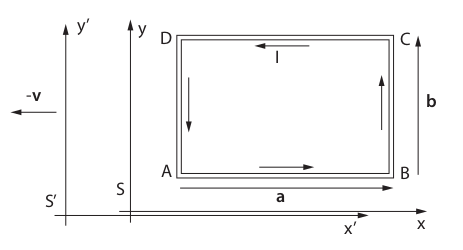
\includegraphics[width=0.7\textwidth]{currentloop.png}
	\caption{Illustration of current loop.}
	\label{fig:currentloop}
\end{figure}

Since the charge density in rest frame $S$ is zero, $\rho(\va{r}) = 0$, the electric dipole moment must also be zero, $\va{p} = 0$.

The current along every edge of the rectangle will be $j\va{n}$, where $\va{n}$ is a unit vector pointing along the edge in question.
\begin{align*}
\text{AB}: \va{j} =j\va{e}_x &\quad \text{BC}: \va{j} =j\va{e}_y \\
\text{CD}: \va{j} =-j\va{e}_x &\quad \text{DA}: \va{j} =-j\va{e}_x.
\end{align*}
Given a point $\va{r}$ along the AB segment,
\begin{equation}
\label{eq:cross1}
\va{r}\cp\va{j}(\va{r}) = (x\va{e}_x + y\va{e}_y)\cp(j\va{e}_x) = -yj\va{e}_z,
\end{equation}
along the BC segment,
\begin{equation}
\label{eq:cross2}
\va{r}\cp\va{j}(\va{r}) = (x\va{e}_x + y\va{e}_y)\cp(j\va{e}_y) = xj\va{e}_z,
\end{equation}
along the CD segment,
\begin{equation}
\label{eq:cross3}
\va{r}\cp\va{j}(\va{r}) = (x\va{e}_x + y\va{e}_y)\cp(-j\va{e}_x) = yj\va{e}_z,
\end{equation}
and along the DA segment
\begin{equation}
\label{eq:cross4}
\va{r}\cp\va{j}(\va{r}) = (x\va{e}_x + y\va{e}_y)\cp(-j\va{e}_y) = -xj\va{e}_z,
\end{equation}

It is a reasonable approximation to use the factor $\Delta$, which is the cross-sectional area of the current wire, instead of integrating in directions perpendicular to the direction of the conductor. Then the coordinate $\va{r}$ is simply the centre of the conductor. Employing these assumptions/approximations and assigning the lower left corner of the rectangle coordinates $(x_0,y_0)$ and using the results from equations \ref{eq:cross1} \ref{eq:cross2}, \ref{eq:cross3} and \ref{eq:cross4} the magnetic dipole moment is
\begin{align*}
\va{m} &= \frac{1}{2}j\Delta\va{e}_z \left(
-\int_{x_0}^{y_0+a} y_0dx + \int_{y_0}^{y_0+b}(x_0+a)dy +\int_{x_0}^{x_0+a}(y_0+b)dx - \int_{y_0}^{y_0+b}x_0dy
\right) \\
&=\frac{1}{2} I (-y_0a + (x_0 + a)b + (y_0 + b)a - x_0b)\va{e}_z \\
&=abI\va{e}_z.
\end{align*} 
Since $\va{a}$ and $\va{b}$ are orthogonal $\va{a} \cp \va{b} = ab\va{e}_z$, which gives
\begin{equation}
\va{m} = I\va{a} \cp \va{b}.
\end{equation}

\subsection{Length Contraction}
Reference frame $S'$ moves at velocity $\va{v}$ to the right, away from the rest frame $S$. Because the width of the loop is orthogonal to the boost, it remains the same, $b' = b$. 

We have the following Lorentz transformations between the positions of the endpoints of the rectangle in the two reference frames
\begin{align*}
x_a = \gamma(-vt_a' + x_a') \quad x_a' = \gamma(vt_a + x_a) \\
x_b = \gamma(-vt_b' + x_b') \quad x_b' = \gamma(vt_b + x_b).
\end{align*}
The two endpoints must be measured at the same time in reference frame $S'$ to compute the correct length
\begin{align*}
a =x_b - x_a &= \gamma(x_b'- x_a') + \cancel{\gamma v(t_a' - t_b')} \\
			 &= \gamma(x_b'- x_a') = \gamma a'
\end{align*}
which yields
\begin{equation}
a = \frac{1}{\gamma}a'.
\end{equation}

\subsection{Charge of Segments AB and CD}
In reference frame $S$, the segment AB will have current four-vector $J^\mu = (0, j, 0, 0)$. Lorentz transform to reference frame $S'$, which has velocity $-v$ relative to $S$ gives
\begin{align*}
\rho'c = J'^0 = L^0_{\ \nu}J^\nu = \gamma(J^0 + \beta J^1) = \beta\gamma J,
\end{align*}
where $\beta = v/c$. Assuming uniform charge density of the conductor segment gives
\begin{align*}
\rho' = \frac{J'^0}{c} = \frac{j\gamma v}{c^2}.
\end{align*}
To find the total charge one needs simply to multiply with the volume of this conductor segment in reference frama $S'$, $\abs{\va{a}}\Delta = (1/\gamma)a\Delta$
\begin{equation}
Q_{AB}' = V_{AB}'\rho_{AB}' = \frac{1}{\gamma}a\Delta j\gamma \frac{v}{c^2} = I a\frac{v}{c^2}.
\end{equation}

A similiar computation can be made for conductor segment CD, with current four-vector $J^\mu = (0, -j, 0, 0)$.
\begin{align*}
\rho'c &= J'^0 = L^0_{\ \nu} J^\nu = \gamma(J^0+ \beta J^1) = -\gamma\beta j \\
\rightarrow \rho' &= \frac{J'^0}{c} = -\frac{\gamma\beta j}{c} = -\frac{\gamma v j}{c^2} \\
\end{align*}
\begin{equation}
Q_{CD}' = V_{CD}'\rho_{CD}' = -\frac{1}{\gamma}a\Delta \gamma j\frac{ v}{c^2} = -Ia\frac{v}{c^2}
\end{equation}

\subsection{Electric and Magnetic Dipole Moment in $S'$}
Segments AB and CD always have charge densities $\rho = \pm\frac{I}{\Delta}\frac{v}{c^2}$. Inserting this into the $\va{p}$ from \ref{eq:edm&mdm} and assuming a thin conductor by replacing the cross-sectional integration dimensions with $\Delta$ gives
\begin{align*}
\va{p}'  &= \int\va{r}\rho(\va{r})d^3r \\
		&= \frac{I}{\cancel{\Delta}}\frac{v}{c^2}
		\left[
		 \cancel{\Delta}\int_{x_0}^{x_0+a}(\cancel{x\va{e}_x} + y_0\va{e}_y)dx 
		-\cancel{\Delta}\int_{x_0}^{x_0+a}(\cancel{x\va{e}_x} + (y_0 + b)\va{e}_y)dx 
		\right] \\
		&= I \frac{v}{c^2}\left(
		\cancel{y_0 x\Big|_{x_0}^{x_0 + a}}
		-(\cancel{y_0} + b)x\Big|_{x_0}^{x_0 + a}
		\right)\va{e}_y \\
		&= I \frac{v}{c^2}\left(-b(x_0 + a - x_0)\right)\va{e}_y \\
		&= -I\frac{v}{c^2}ab\va{e}_y
\end{align*}
Moreover
\begin{align*}
-\frac{1}{c^2}\va{m} \cp \va{v} &= -\frac{1}{c^2}(abI\va{e}_z) \cp (v\va{e}_x) \\
			&= -\frac{v}{c^2}Iab (\va{e}_z \cp \va{e}_x) \\
			&= -I \frac{v}{c^2}ab\va{e}_y,
\end{align*}
which implies that
\begin{equation}
\va{p}' = - \frac{1}{c^2}\va{m} \cp \va{v}
\end{equation}

In order to calculate the magnetic dipole moment, one needs the current densities for all conductor segments.
\begin{align*}
\text{AB:} &\ J = (0, j, 0, 0) \quad j' = J'^1 = \beta\gamma J^0 + \gamma J^1 = \gamma j \\
\text{CD:} &\ J = (0, -j, 0, 0) \quad j' = J'^1 = \beta\gamma J^0 + \gamma J^1 = -\gamma j.
\end{align*}
Segments AB and CD both have current densities $j' = \gamma j$ in $x$-direction. Segments BA and DA have current density $j$ unchanged. However, the width of these conductors are Lorentz-contracted, meaning that the area is reduced by a factor $\gamma^{-1}$, so that $\Delta' = \Delta / \gamma$. Now to compute the magnetic dipole moment in the same manner as before
\begin{align*}
\va{m}' &= \frac{1}{2}\va{e}_z\left[
	\gamma j \Delta \int_{x_0'}^{x_0' + a'} (\cancel{y_0} + b - \cancel{y_0})dx' 
	j \frac{\Delta}{\gamma} \int_{y_0'}^{y_0' + b'} (\cancel{x_0'} + a - \cancel{x_0'})
	\right] \\
	&= \frac{1}{2} j \Delta ab (1 + \gamma^{-2})\va{e}_z = \frac{1}{2} I ab (2 - \beta^2)\va{e}_z = I ab (1 - \frac{\beta^2}{2})\va{e}_z
\end{align*}
\begin{equation}
\va{m}' = \left(1 - \frac{\beta^2}{2} \right)\va{m}
\end{equation}

\subsection{Current in the Different Segments}
The current density is $j' = \gamma j$ in AB and CD, while the cross-sectional area is unchanged. This makes the current
\begin{equation}
I' = \Delta j^1 = \gamma\Delta j = \gamma I.
\end{equation}

For BC and DA $j' = j$, but $\Delta' = \Delta / \gamma$, so
\begin{equation}
I' = \Delta'j = \frac{\Delta}{\gamma}j = \frac{I}{\gamma}
\end{equation}

\end{document}